\chapter{Materials and Method}
\label{cha:materials_and_method}

\section{Dataset}
\label{sec:dataset}

\subsection{Creation}
\label{subsec:creation}

We created our used dataset from approximately 3000 scientific articles in pdf format. An important point was that these articles contained various information, and thereby we ensured that they come from different scientific fields. To be able to use the data we had to separate them from the pdfs and add additional information first.

We used a text mining pre-processing technique as introduced by Vijayarani et al.~\cite{Vijayarani2015} to separate the data from the pdf. This technique consists of three key steps, which are called the extraction-, the stopwords removal-, and the stemming-step. At first we seperated the article structure, and the raw text from the pdf. For those we used a framework descriped in \Cref{subsec:extract_document_structure}. The stopwords removal-, and the stemming step was done as descriped in \cref{subsec:stop_words} and \Cref{subsec:stemming} (TODO: more detailed).

TODO: Write about the imrad type of an chapter - describe why each section can have severeal imrad types

At last we performed a semi-automated annotation to link the references of the scientific articles. Thereby similarities about the references of an article and the titles of all other articles are compared as described in \Cref{sec:text_similarities}, and if they exceed a given threshold a recommentation to create a link between those two was given.

We created each data record in such a way that it can be transferred directly to the database schema showen in \Cref{fig:database_schema}. To reduce noise during the evaluation we removed all articles without any connection to other articles, so we had 821 scientific articles in our final dataset.

\myfig{database_schema}
      {width=0.70\textwidth}
      {Database Schema for the used Dataset}
      {Database Schema for the used Dataset}
      {fig:database_schema}

\subsection{Structure of a Scientific Article}
\label{sec:structure_scientific_article}

When looking at the scientific article in the database schema in \Cref{fig:database_schema} there are various member attributes. The first important point is that all text values are available raw and processed. The term raw stands for the text being saved as it was separated. Processed text is the raw text after the stopword removal-, and the stemming step.

The author text attribute contains the names and email adresses of all authors. Thereby this attribute has three values. The complete text, the text reduced to emails, and a list of all authors. This part of the article is the only one that is not preprocessed.

\myfig{scientific_articles_tree}
      {width=0.90\textwidth}
      {Scientific Article represended as a Tree}
      {Scientific Article represended as a Tree}
      {fig:scientific_articles_tree}

One of the most important characteristics are the sections, and the underlying structure that comes with it. \Cref{fig:scientific_articles_tree} showes that scientific articles are structured like a tree. It is easy to see that the chapters are non-leaf nodes, and text areas are the leaf nodes. This is reflected in database schema with two lists. One for the subsections, and one for text areas. In addition to the lists, each section itself has a section type. This attribute reflects whether the section is a section, subsection, or subsubsection. The IMRaD structure information is stored as the IMRaD type. As described in \Cref{subsec:creation}, each section can have several IMRaD types, and each type of section holds its own list of these types.

We stored word histograms for the article, and the sections so we dont have to discover the complete text for each search request. These histograms contain the term frequencies of the underlying area. So the subsubsections contain the frequencies of their text areas, the subsections contain the frequencies of their text areas, and their subsubsections text areas, and so on. Finally the article holds all term frequencies of the whole document.

The last two attributes of the article are the reference-, and the cited-by-list. If an id is set in the reference, the referenced paper has an entry in the cited-by-list. Additional we stored the text of whole reference, the authors, and other available information like publisher, pages, volume, etc.

\subsection{Citation Network}
\label{sec:citation_network}

\myfig{dataset_generall}
      {width=0.50\textwidth}
      {General Structure of a Citation Network}
      {General Structure of a Citation Network}
      {fig:structure_citation_network}

Citation networks represent the relationships inside a set of scientific articles. \Cref{fig:structure_citation_network} shows the structure, and the properties ~\cite{kas2011} of such a network. Therby the articles regards as nodes, and an edge from node i to node j is added if i cites j. The timeline indicates that new articles citing existing articles, and thus there can not be cyclic dependencies.

\begin{table}
  \centering
  \begin{tabular}{ l c }
    \toprule
    \textbf{Number of Nodes}      & $821$  \\ \midrule
    \textbf{Number of Edges}      & $1716$ \\ \midrule
    \textbf{Number of Strongly Connected Components} & $821$    \\ \midrule
    \textbf{Number of Cycles}     & $0$    \\ \midrule
    \textbf{Longest Path}         & $12$   \\ \midrule
    \textbf{Number of Root Nodes} & $107$  \\
    \bottomrule
  \end{tabular}
  \caption[General Properties about the citation network]{General Properties about the citation network}
  \label{tbl:general_properties_about_the_graph}
\end{table}

The main properties of our citation network are shown at \Cref{tbl:general_properties_about_the_graph}(TODO: describe importat points).

%Three important points about the network
%One important point is that there are no cycles, which can be also seen by the number of strongly connected components. The longest citation chain over the timeline is defined by the longest path.%

\begin{figure}
  \begin{floatrow}

    \capbtabbox[4.6cm][6cm]{
      \begin{tabular}{ l c }
        \toprule
        \textbf{Max Degree}    & $98$     \\ \midrule
        \textbf{Mean Degree}   & $5.8767$ \\ \midrule
        \textbf{Median Degree} & $2$      \\
        \bottomrule
      \end{tabular}
    }{
      \label{tbl:properties_ingoing_edges}
      \caption[Properties of the Citation Networks In-Degree Distribution]{Properties of the In-Degree Distribution}
    }

    \ffigbox[12cm][5.5cm]{
      {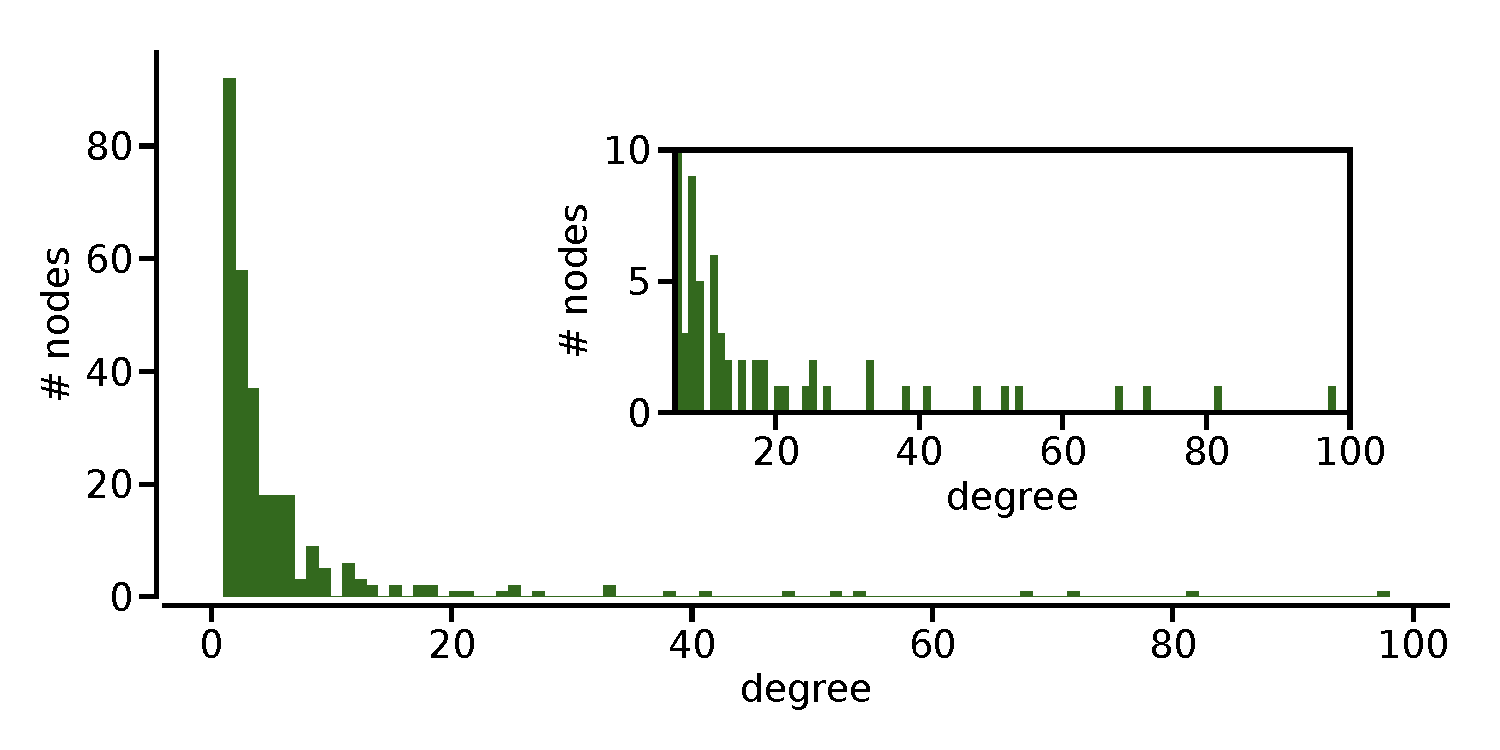
\includegraphics[width=0.70\textwidth]{figures/in-degree_distribution}}
    }{
      \label{fig:indegree_distribution}
      \caption[In-Degree Distribution in the Citation Network]{In-Degree Distribution}
    }
  \end{floatrow}
\end{figure}


The in-degree distribution and their properties How is it represented (citations to papers)

\begin{figure}
  \begin{floatrow}
    \capbtabbox[4.8cm][6cm]{
      \begin{tabular}{ l c }
        \toprule
        \textbf{Max Degree}    & $13$     \\ \midrule
        \textbf{Mean Degree}   & $2.4034$ \\ \midrule
        \textbf{Median Degree} & $2$      \\
        \bottomrule
      \end{tabular}
    }{
      \label{tbl:properties_ingoing_edges}
      \caption[Properties of the Citation Networks Out-Degree Distribution]{Properties of the Out-Degree Distribution}
    }

    \ffigbox[12cm][5.5cm]{
      {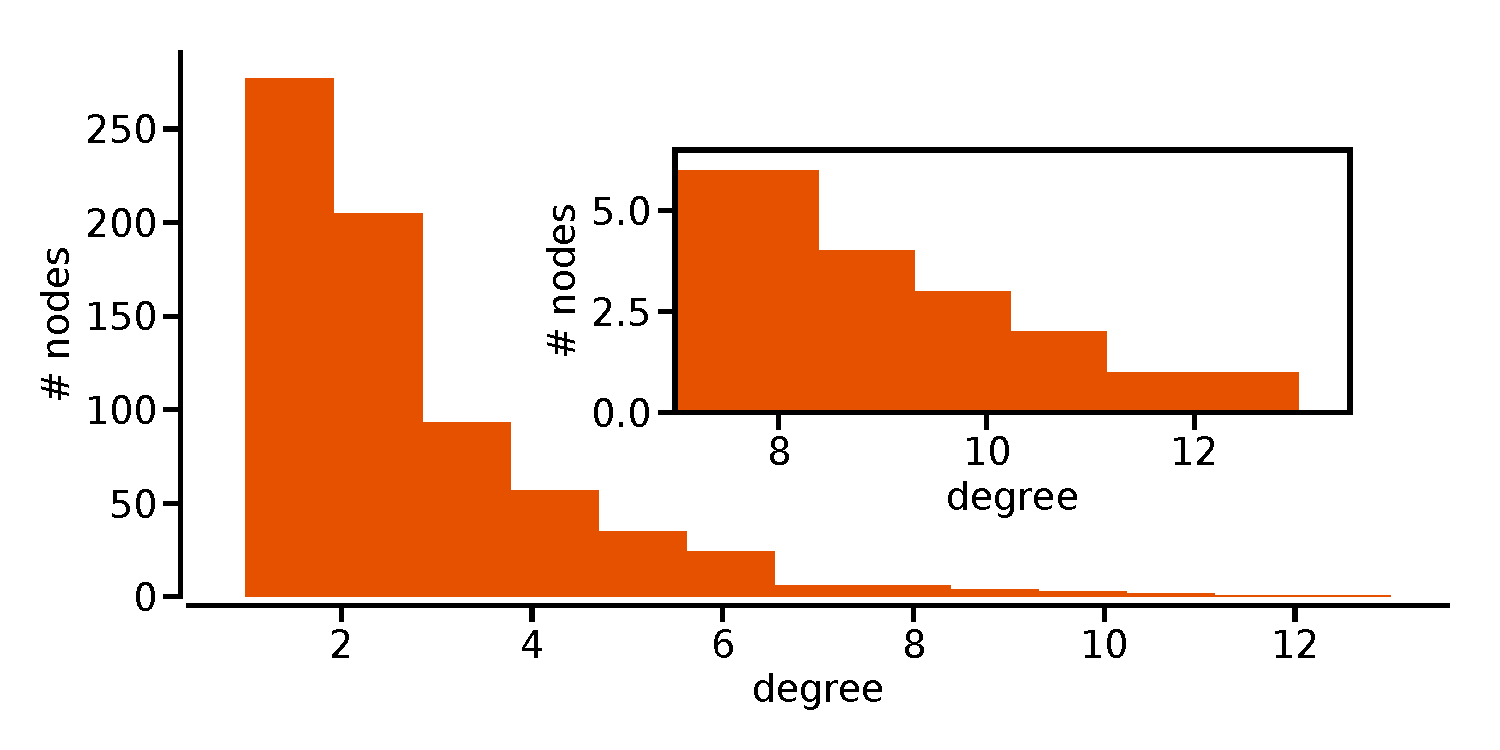
\includegraphics[width=0.7\textwidth]{figures/out-degree_distribution}}
    }{
      \label{fig:outdegree_distribution}
      \caption[Out-Degree Distribution in the Citation Network]{Out-Degree Distribution}
    }
  \end{floatrow}
\end{figure}

The out-degree distribution and their properties How is it represented (citations to papers)

\subsubsection{Data cleaning}
\label{subsubsec:data_cleaning}
Write something about the cycles in the network. preprints cite each other, and why they are removed for the network.

\myfig{preprint_problem}
      {width=0.30\textwidth}
      {Cyclic dependency in a directed graph}
      {Cyclic dependency in a directed graph}
      {fig:preprint_problem}

\section{Model}
\label{sec:model}

Write general about information retrieval models as descriped in ~\cite{ModernInvormationRetrieval1999} page 57

\subsection{Query Structure}

Write how a query looks like - explizit and implizit

\subsection{Introducing IMRaD Structure Features into Weighing Schemes}

Write how the algorithms described in \cref{sec:ranking_algorithms} are modified for imrad structure features.
